\documentclass[a4paper,8pt,twocolumn]{article}
\usepackage[UTF8]{ctex}
\usepackage{graphicx}
\usepackage{fancyhdr}
\usepackage{amsmath}
\usepackage{subcaption}
\usepackage{float}
\usepackage[
  left=2cm,
  right=2cm,
  top=1.5cm,
  bottom=2.5cm
]{geometry}
\usepackage{siunitx}
\usepackage{booktabs}
\usepackage{enumitem}
\usepackage{array}
\usepackage{tabularx}
\newcolumntype{Y}{>{\centering\arraybackslash}X}
\usepackage{amssymb}
\usepackage{pgfplots}
\usepackage{pgfplotstable}
\pgfplotsset{compat=1.18}
\usepackage{tikz}

\sisetup{
  per-mode=symbol,
  separate-uncertainty = true
}

\title{
  \textbf{\huge 塞曼效应}
}
\author{
  \small 中山大学物理学院~广东~广州
}

\pagestyle{fancy}
\fancyhf{}
\fancyhead[C]{塞曼效应}
\fancyfoot[C]{\thepage}

\begin{document}
\maketitle
\newpage

%%%%%%%%%%%%%%%%%%%%%%%%%%%%%%%%%%%%%%%%%%%%%%%%%%%%%%%%%%%%
\section{实验目的}

\begin{enumerate}
  \item 掌握塞曼效应的基本理论，理解原子能级在外磁场中的分裂规律；
  \item 掌握法布里—珀罗（F-P）标准具的工作原理及调节方法；
  \item 观察汞灯谱线的反常塞曼效应（\SI{546.1}{nm}）和正常塞曼效应（\SI{579.06}{nm}）；
  \item 利用干涉圆环的直径数据测定电子的荷质比$e/m$，并与理论值进行比较。
\end{enumerate}

%%%%%%%%%%%%%%%%%%%%%%%%%%%%%%%%%%%%%%%%%%%%%%%%%%%%%%%%%%%%
\section{实验仪器与装置}

\begin{itemize}
  \item 电磁铁及直流稳压电源（电流范围\SIrange{0}{6}{A}）；
  \item 笔形汞灯（Hg）光源；
  \item 会聚透镜；
  \item 干涉滤光片（中心波长\SI{546.1}{nm}用于反常塞曼效应；中心波长\SI{590}{nm}、带宽$\pm\SI{5}{nm}$用于正常塞曼效应）；
  \item 法布里—珀罗标准具（间距$d=\SI{2.05}{mm}$）；
  \item 偏振片；
  \item CCD相机及图像采集系统；
  \item 毫特斯拉计（用于磁场标定）。
\end{itemize}

%%%%%%%%%%%%%%%%%%%%%%%%%%%%%%%%%%%%%%%%%%%%%%%%%%%%%%%%%%%%
\section{实验原理}

\subsection{原子的磁矩与朗德因子}

在LS耦合下，原子的总磁矩$\mu_J$与总角动量$P_J$的关系为
\begin{equation}
  \mu_J = g\frac{e}{2m}P_J
  \tag{1}
\end{equation}
其中$g$为朗德因子：
\begin{equation}
  g = 1 + \frac{J(J+1)+S(S+1)-L(L+1)}{2J(J+1)}
  \tag{2}
\end{equation}

\subsection{外磁场中的能级分裂}

在外磁场$B$中，原子获得附加能量
\begin{equation}
  \Delta E = Mg\mu_B B
  \tag{3}
\end{equation}
其中$\mu_B = eh/(4\pi m)$为玻尔磁子，$M$为磁量子数，取值$M = J, J-1, \ldots, -J$，共$2J+1$个值。原来简并的能级分裂为$2J+1$个子能级。

\subsection{塞曼效应的选择定则与谱线分裂}

磁场中两能级间跃迁产生的谱线与原谱线的波数差为
\begin{equation}
  \Delta\tilde{\nu} = (M_2 g_2 - M_1 g_1)\,\tilde{L}
  \tag{4}
\end{equation}
其中$\tilde{L} = eB/(4\pi mc)$为洛伦兹单位。跃迁选择定则为：
\begin{itemize}
  \item $\Delta M = 0$：$\pi$线，光振动平行于磁场方向的线偏振光；
  \item $\Delta M = \pm 1$：$\sigma$线，光振动垂直于磁场的线偏振光。
\end{itemize}

\textbf{反常塞曼效应}（Hg \SI{546.1}{nm}，${}^3S_1 \to {}^3P_2$）：

上能级${}^3S_1$：$L=0, S=1, J=1$，$g_2 = 2$；下能级${}^3P_2$：$L=1, S=1, J=2$，$g_1 = 3/2$。

$\pi$分量（$\Delta M = 0$）：
\begin{equation}
  \Delta\tilde{\nu}_\pi = M(g_2 - g_1)\tilde{L} = \frac{M}{2}\tilde{L},\quad M = -1,0,1
  \tag{5}
\end{equation}
三条$\pi$线位于$-\frac{1}{2}\tilde{L},\; 0,\; +\frac{1}{2}\tilde{L}$，相邻间距为$\frac{1}{2}\tilde{L}$。

$\sigma$分量（$\Delta M = \pm 1$）共6条线，位于$\pm\tilde{L},\; \pm\frac{3}{2}\tilde{L},\; \pm 2\tilde{L}$，共计9条分裂谱线。

\textbf{正常塞曼效应}（Hg \SI{579.06}{nm}，${}^1D_2 \to {}^1P_1$）：

两能级均为单重态，$S=0$，$g_1 = g_2 = 1$。上下能级在磁场中分裂间隔相等，所有相同$\Delta M$的跃迁重合，仅分裂为三条谱线，$\sigma$与$\pi$的间距恰好为一个洛伦兹单位$\tilde{L}$。

\subsection{法布里—珀罗标准具}

F-P标准具的干涉极大条件为
\begin{equation}
  2d\cos\theta = N\lambda
  \tag{6}
\end{equation}
其中$d$为标准具间距，$\theta$为入射角，$N$为干涉序。在扩展光源照明下产生等倾干涉圆环。

自由光谱范围：
\begin{equation}
  \Delta\lambda_F = \frac{\lambda^2}{2d}
  \tag{7}
\end{equation}

精细度：
\begin{equation}
  F = \frac{\pi\sqrt{R}}{1-R}
  \tag{8}
\end{equation}
其中$R$为反射面的反射率。

\subsection{测量电子荷质比的公式}

利用透镜将干涉条纹成像于焦平面上，对同一波长相邻两序的条纹直径平方差为
\begin{equation}
  \Delta D^2 = D_{N-1}^2 - D_N^2 = \frac{4f^2\lambda}{d}
  \tag{9}
\end{equation}

对同一序不同波长的两条干涉环，其波数差为
\begin{equation}
  \Delta\tilde{\nu} = \frac{D_b^2 - D_a^2}{2d\,\Delta D^2}
  \tag{10}
\end{equation}
其中$D_a$、$D_b$分别为同一序中两分裂分量的直径，$\Delta D^2 = D_{N-1}^2 - D_b^2$。

对于\textbf{反常塞曼效应}，用偏振片选取$\pi$分量观测，相邻$\pi$线间距$\Delta\tilde{\nu} = \frac{1}{2}\tilde{L}$，代入$\tilde{L} = eB/(4\pi mc)$得
\begin{equation}
  \frac{e}{m} = \frac{4\pi c\,(D_b^2 - D_a^2)}{d\,B\,\Delta D^2}
  \tag{11}
\end{equation}

对于\textbf{正常塞曼效应}，直接观测$\sigma$与$\pi$分量，间距$\Delta\tilde{\nu} = \tilde{L}$，得
\begin{equation}
  \frac{e}{m} = \frac{2\pi c\,(D_b^2 - D_a^2)}{d\,B\,\Delta D^2}
  \tag{12}
\end{equation}

%%%%%%%%%%%%%%%%%%%%%%%%%%%%%%%%%%%%%%%%%%%%%%%%%%%%%%%%%%%%
\section{实验内容与步骤}

\subsection{磁场强度与电流的标定}

由于实验过程中无法同时测量磁场与观测干涉环，需事先标定电磁铁磁场强度$B$与通电电流$I$的关系。将特斯拉计探头平置于磁极间隙中心，缓慢转动使读数最大，在$I = \SIrange{0}{5.6}{A}$范围内逐步测量$B$值。

\subsection{反常塞曼效应的观测（\SI{546.1}{nm}）}

光路依次为：Hg灯\,$\to$\,会聚透镜\,$\to$\,干涉滤光片（\SI{546.1}{nm}）\,$\to$\,F-P标准具\,$\to$\,偏振片\,$\to$\,CCD相机。

\begin{enumerate}[label=(\arabic*)]
  \item 不加磁场，调整光路使各元件等高共轴，并以磁极间隙中心为等高基准；
  \item 用肉眼确认F-P标准具上出现干涉圆环后，安装CCD相机，调整光圈、焦距及放大倍数，使圆环清晰锐利且无过曝；
  \item 旋转偏振片选取$\pi$分量，在$I = \SIrange{4.0}{5.0}{A}$范围内取三个电流值；
  \item 用鼠标在屏幕上读取干涉圆环的相对直径$D_a$、$D_b$和$D_{N-1}$，代入式(11)计算$e/m$。
\end{enumerate}

\subsection{正常塞曼效应的观测（\SI{579.06}{nm}）}

光路改为：Hg灯\,$\to$\,会聚透镜\,$\to$\,窄带滤光片（中心\SI{590}{nm}）\,$\to$\,F-P标准具\,$\to$\,CCD相机。不使用偏振片。

由于\SI{579.06}{nm}谱线可能受\SI{576.96}{nm}反常谱线的干扰（两者间距仅\SI{2.1}{nm}，在滤光片$\pm\SI{5}{nm}$带宽内），需要将滤光片偏转约$16^\circ$使中心波长蓝移。操作时先偏转至同时看到两组圆环，再反向微调至只剩\SI{579.06}{nm}的清晰圆环。

在$I = \SIrange{2.4}{3.8}{A}$范围内取三个电流值，读取$D_a$、$D_b$和$D_{N-1}$，代入式(12)计算$e/m$。

%%%%%%%%%%%%%%%%%%%%%%%%%%%%%%%%%%%%%%%%%%%%%%%%%%%%%%%%%%%%
\section{实验结果与分析}
\label{sec:results}

\subsection{磁场标定结果}

图\,\ref{fig:calibration}\,为磁场强度$B$与通电电流$I$的标定曲线。在$I < \SI{2}{A}$时$B$与$I$近似线性，斜率约为$\SI{323}{mT/A}$；当$I > \SI{3}{A}$后磁芯逐渐饱和，曲线明显弯曲。

\begin{figure}[H]
  \centering
  \begin{tikzpicture}
  \begin{axis}[
      width=0.92\columnwidth,
      height=0.22\textheight,
      scale only axis,
      grid=major,
      xlabel={电流 $I$ / A},
      ylabel={磁感应强度 $B$ / mT},
      title style={font=\small},
      label style={font=\small},
      ticklabel style={font=\scriptsize},
      xmin=0, xmax=5.8,
      ymin=0, ymax=1400,
      mark size=1.2pt
  ]
    \addplot[mark=*,blue,thick] coordinates {
      (0,0)(0.2,53)(0.4,113)(0.6,177)(0.8,243)
      (1.0,312)(1.2,380)(1.4,448)(1.6,515)(1.8,581)
      (2.0,646)(2.2,708)(2.4,769)(2.6,827)(2.8,882)
      (3.0,933)(3.2,981)(3.4,1025)(3.6,1064)(3.8,1100)
      (4.0,1133)(4.2,1163)(4.4,1191)(4.6,1216)(4.8,1240)
      (5.0,1263)(5.2,1283)(5.4,1302)(5.6,1321)
    };
  \end{axis}
  \end{tikzpicture}
  \caption{磁场强度$B$与电流$I$的标定曲线}
  \label{fig:calibration}
\end{figure}

\subsection{Hg灯谱线}

图\,\ref{fig:hg}\,为Hg灯的发射谱图，可见本实验所关注的两条谱线$\SI{546.08}{nm}$和$\SI{579.07}{nm}$以及邻近的$\SI{576.96}{nm}$谱线。

\begin{figure}[H]
  \centering
  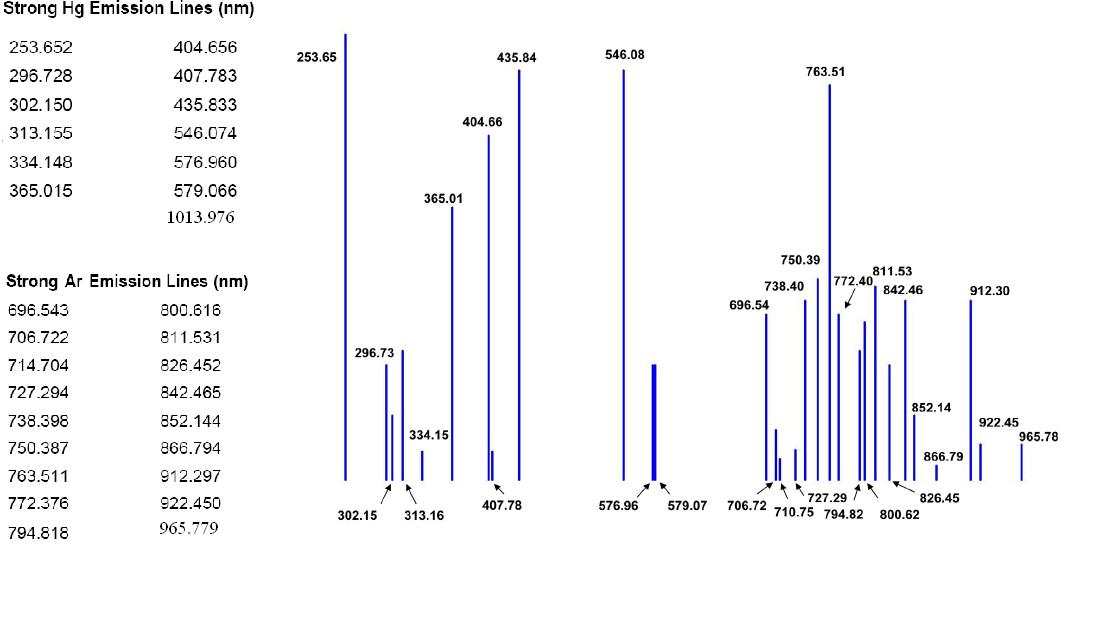
\includegraphics[width=0.95\columnwidth]{Hg谱图2.jpg}
  \caption{Hg灯发射光谱}
  \label{fig:hg}
\end{figure}

\subsection{反常塞曼效应（\SI{546.1}{nm}）}

\subsubsection{能级分裂与跃迁图}

\SI{546.1}{nm}谱线对应${}^3S_1 \to {}^3P_2$跃迁。上能级（$J=1,\,g=2$）分裂为3个子能级，下能级（$J=2,\,g=3/2$）分裂为5个子能级，按选择定则$\Delta M = 0, \pm 1$共产生9条分裂谱线。

谱线位移（以$\tilde{L}$为单位）如下：
\begin{itemize}
  \item $\sigma^-$成分：$-2,\; -\dfrac{3}{2},\; -1$
  \item $\pi$成分：$-\dfrac{1}{2},\; 0,\; +\dfrac{1}{2}$
  \item $\sigma^+$成分：$+1,\; +\dfrac{3}{2},\; +2$
\end{itemize}

\subsubsection{干涉圆环图像}

图\,\ref{fig:anomalous}\,展示了在不同电流下观测到的$\pi$分量干涉圆环。可以看到每个原始圆环分裂为三个子环。

\begin{figure}[H]
  \centering
  \begin{subfigure}[b]{0.31\columnwidth}
    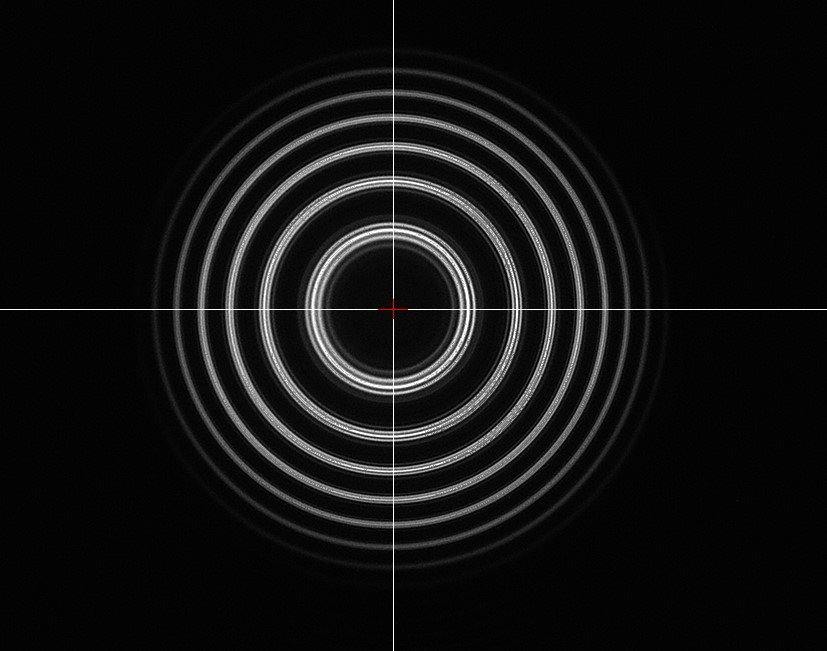
\includegraphics[width=\textwidth]{反常4.0A.jpg}
    \caption{$I=\SI{4.0}{A}$}
  \end{subfigure}
  \hfill
  \begin{subfigure}[b]{0.31\columnwidth}
    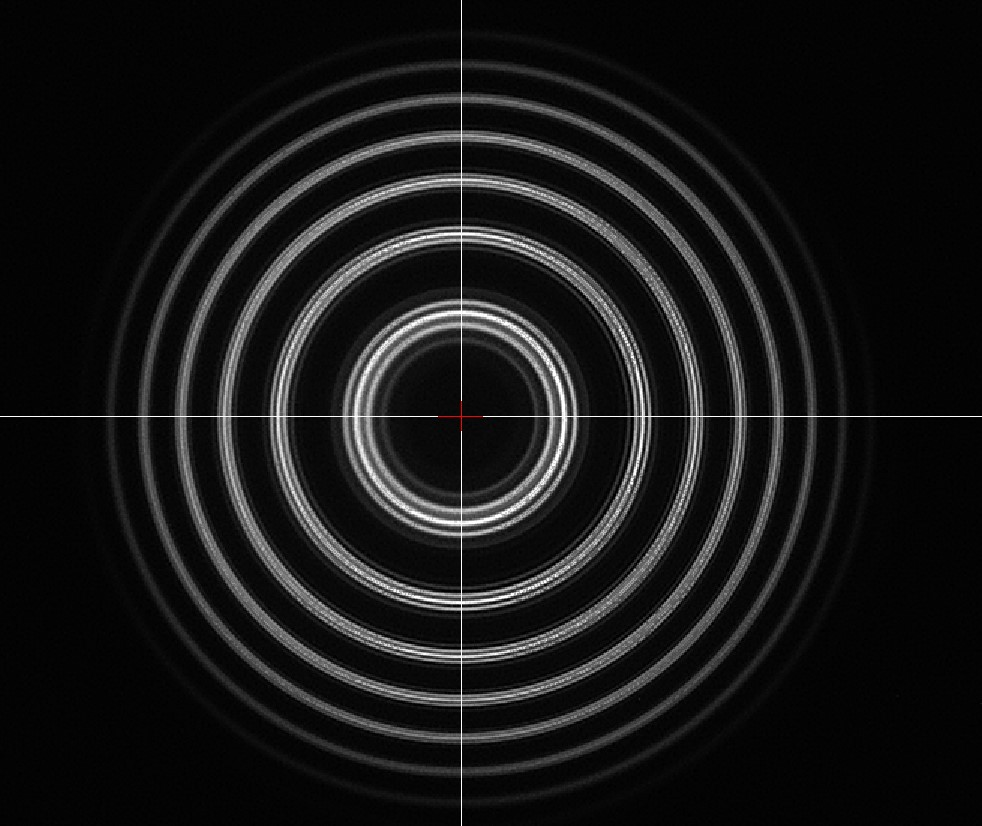
\includegraphics[width=\textwidth]{反常4.2A.jpg}
    \caption{$I=\SI{4.2}{A}$}
  \end{subfigure}
  \hfill
  \begin{subfigure}[b]{0.31\columnwidth}
    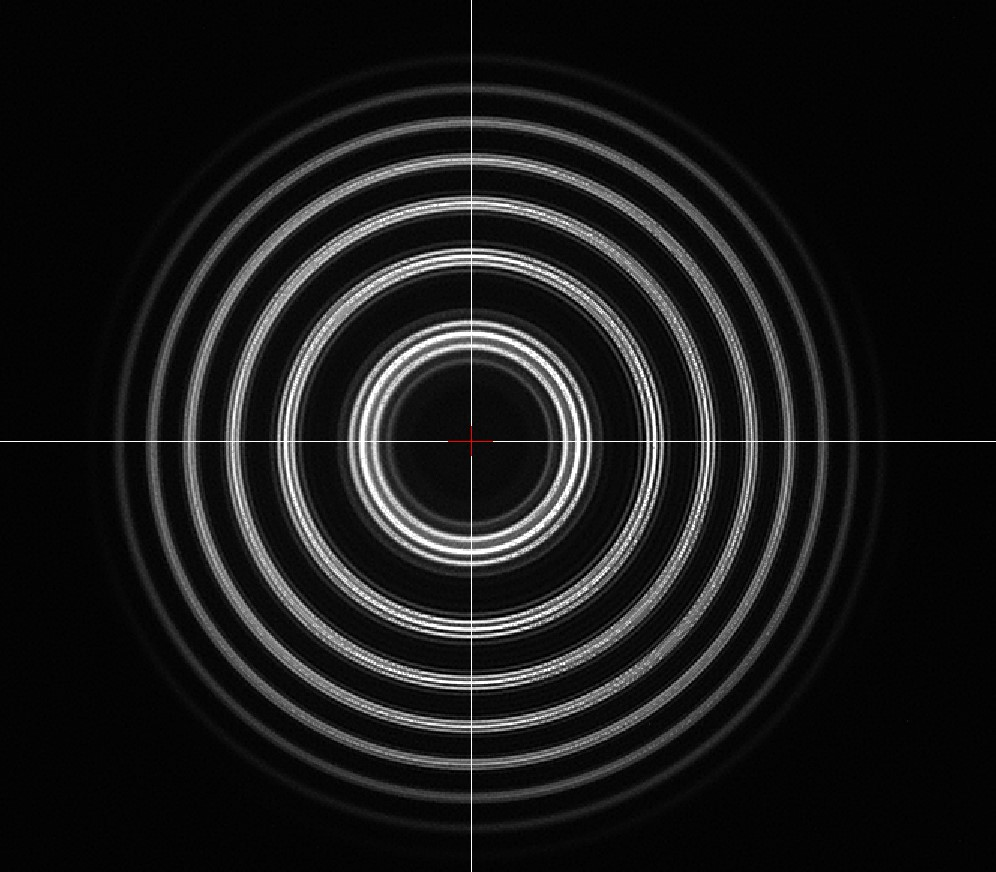
\includegraphics[width=\textwidth]{反常5.0A.jpg}
    \caption{$I=\SI{5.0}{A}$}
  \end{subfigure}
  \caption{反常塞曼效应干涉圆环（$\pi$分量，\SI{546.1}{nm}）}
  \label{fig:anomalous}
\end{figure}

\subsubsection{数据处理与$e/m$计算}

使用式(11)计算电子荷质比，其中$d = \SI{2.05}{mm}$，$c = \SI{2.998e8}{m/s}$，$B$由标定曲线查得。$D_a$、$D_b$为同一序中相邻$\pi$线的直径（像素），$\Delta D^2 = D_{N-1}^2 - D_b^2$。结果列于表\,\ref{tab:anomalous}。

\begin{table}[H]
\centering
\caption{反常塞曼效应$e/m$测量结果}
\label{tab:anomalous}
\begin{tabularx}{\columnwidth}{YYYYYY}
\toprule
$I$/A & $B$/mT & $D_a$ & $D_b$ & $D_{N\!-\!1}$ & \makebox[0pt][c]{\scriptsize$e/m\;(10^{11}\text{C/kg})$} \\
\midrule
4.2 & 1163 & 122 & 139 & 243 & 1.765 \\
4.0 & 1133 & 244 & 252 & 322 & 1.602 \\
5.0 & 1263 & 238 & 247 & 317 & 1.609 \\
\bottomrule
\end{tabularx}
\end{table}

\begin{table}[H]
\centering
\caption{反常塞曼效应相对误差}
\label{tab:anomalous_err}
\begin{tabularx}{\columnwidth}{YYY}
\toprule
$I$/A & \makebox[0pt][c]{\scriptsize$e/m\;(10^{11}\text{C/kg})$} & 相对误差 \\
\midrule
4.2 & 1.765 & $0.34\%$ \\
4.0 & 1.602 & $8.93\%$ \\
5.0 & 1.609 & $8.53\%$ \\
\bottomrule
\end{tabularx}
\end{table}

电子荷质比的理论值为$e/m = \SI{1.759e11}{C/kg}$。$I = \SI{4.2}{A}$时测量值与理论值吻合良好（误差$0.34\%$），而$I = \SI{4.0}{A}$和$\SI{5.0}{A}$时误差较大（约$9\%$），主要原因为线圈通电时间过长导致发热，内阻改变使实际磁场偏离标定值，同时光路偏差也较显著（详见§\,6误差分析）。

\subsection{正常塞曼效应（\SI{579.06}{nm}）}

\subsubsection{能级分裂与跃迁图}

\SI{579.06}{nm}谱线对应${}^1D_2 \to {}^1P_1$跃迁。两能级均为单重态（$S=0$），$g_1 = g_2 = 1$，上下能级分裂间隔相等，所有相同$\Delta M$的跃迁完全重合，仅产生三条谱线：$\sigma^-$（$-\tilde{L}$）、$\pi$（$0$）、$\sigma^+$（$+\tilde{L}$），相邻间距恰为一个洛伦兹单位。

\subsubsection{干涉圆环图像}

图\,\ref{fig:normal}\,展示了正常塞曼效应的干涉圆环。可以观察到每个原始圆环清晰地分裂为三个等间距的子环。

\begin{figure}[H]
  \centering
  \begin{subfigure}[b]{0.31\columnwidth}
    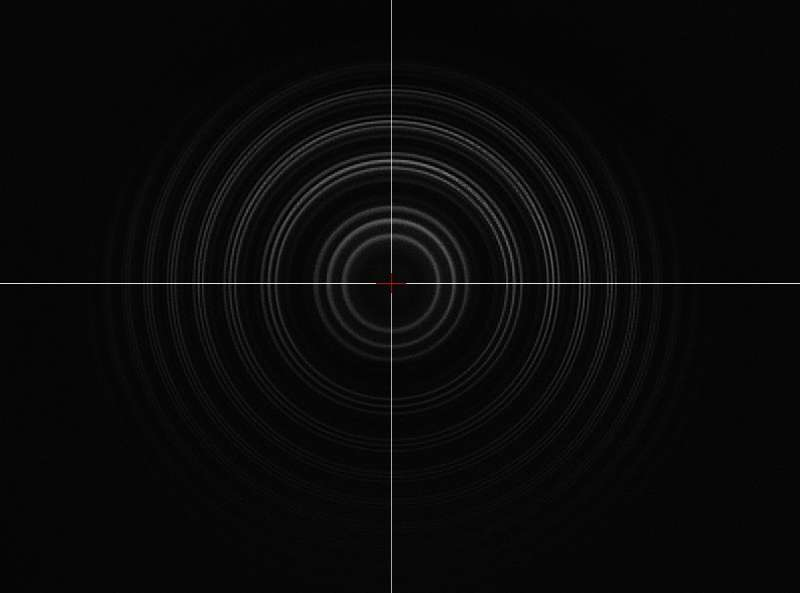
\includegraphics[width=\textwidth]{正常2.4A.jpg}
    \caption{$I=\SI{2.4}{A}$}
  \end{subfigure}
  \hfill
  \begin{subfigure}[b]{0.31\columnwidth}
    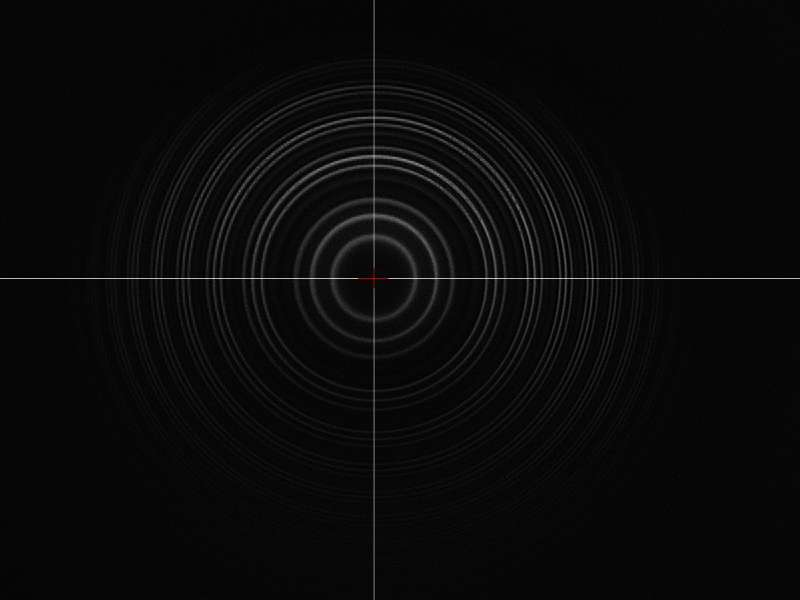
\includegraphics[width=\textwidth]{正常3.4A.jpg}
    \caption{$I=\SI{3.4}{A}$}
  \end{subfigure}
  \hfill
  \begin{subfigure}[b]{0.31\columnwidth}
    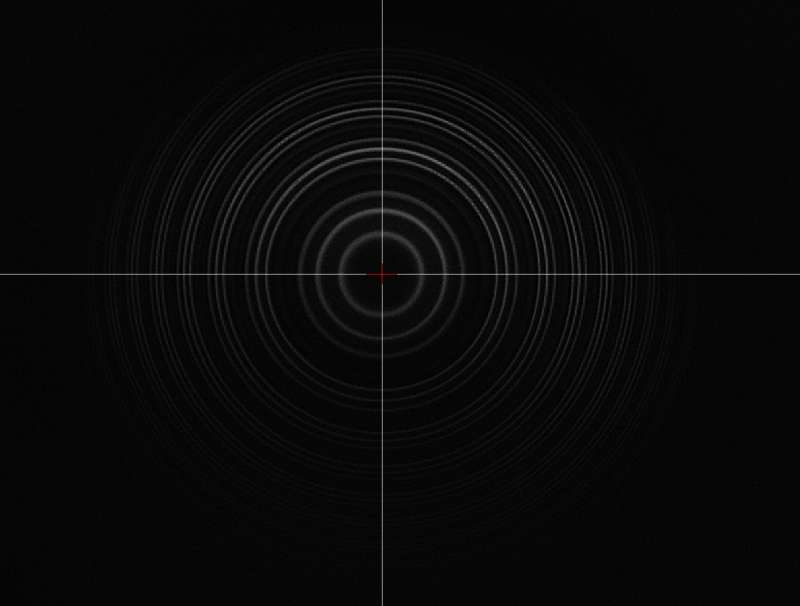
\includegraphics[width=\textwidth]{正常3.8A.jpg}
    \caption{$I=\SI{3.8}{A}$}
  \end{subfigure}
  \caption{正常塞曼效应干涉圆环（\SI{579.06}{nm}）}
  \label{fig:normal}
\end{figure}

\subsubsection{数据处理与$e/m$计算}

使用式(12)计算，其中$D_a$为$\pi$分量的直径，$D_b$为$\sigma$分量的直径，$\Delta D^2 = D_{N-1}^2 - D_b^2$。注意正常塞曼效应无需偏振片即可分辨三个分量。滤光片偏转$16^\circ$以排除\SI{576.96}{nm}谱线干扰。结果列于表\,\ref{tab:normal}。

\begin{table}[H]
\centering
\caption{正常塞曼效应$e/m$测量结果}
\label{tab:normal}
\begin{tabularx}{\columnwidth}{YYYYYY}
\toprule
$I$/A & $B$/mT & $D_a$ & $D_b$ & $D_{N\!-\!1}$ & \makebox[0pt][c]{\scriptsize$e/m\;(10^{11}\text{C/kg})$} \\
\midrule
3.8 & 1100 & 84 & 128 & 245 & 1.785 \\
3.4 & 1025 & 83 & 124 & 243 & 1.742 \\
2.4 & 769  & 94 & 125 & 244 & 1.847 \\
\bottomrule
\end{tabularx}
\end{table}

\begin{table}[H]
\centering
\caption{正常塞曼效应相对误差}
\label{tab:normal_err}
\begin{tabularx}{\columnwidth}{YYY}
\toprule
$I$/A & \makebox[0pt][c]{\scriptsize$e/m\;(10^{11}\text{C/kg})$} & 相对误差 \\
\midrule
3.8 & 1.785 & $1.51\%$ \\
3.4 & 1.742 & $0.95\%$ \\
2.4 & 1.847 & $5.03\%$ \\
\bottomrule
\end{tabularx}
\end{table}

利用测量数据可以直接计算塞曼分裂间隔。由式(10)得$\sigma$-$\pi$波数差$\Delta\tilde{\nu}_{\text{exp}}$，同时可换算为波长差$\delta\lambda = \lambda^2\Delta\tilde{\nu}$。理论预期$\tilde{L}_{\text{theo}} = eB/(4\pi mc) = 0.4674\,B$\,(cm$^{-1}$，$B$以T为单位），其中$e/m$取标准值$\SI{1.759e11}{C/kg}$。结果列于表\,\ref{tab:splitting}。

\begin{table}[H]
\centering
\caption{正常塞曼效应分裂间隔（$\sigma$-$\pi$间距）}
\label{tab:splitting}
\begin{tabularx}{\columnwidth}{YYYYY}
\toprule
$I$/A & $B$/T & $\Delta\tilde{\nu}_{\text{exp}}$/cm$^{-1}$ & $\tilde{L}_{\text{theo}}$/cm$^{-1}$ & $\delta\lambda_{\text{exp}}$/nm \\
\midrule
3.8 & 1.100 & 0.521 & 0.514 & 0.0175 \\
3.4 & 1.025 & 0.474 & 0.479 & 0.0159 \\
2.4 & 0.769 & 0.377 & 0.359 & 0.0126 \\
\bottomrule
\end{tabularx}
\end{table}

实测分裂波长差$\delta\lambda$在$0.013\sim\SI{0.018}{nm}$量级，远小于F-P标准具的自由光谱范围$\Delta\lambda_F = \lambda^2/(2d) = \SI{0.082}{nm}$，说明仪器的分辨能力满足测量需求。实验分裂间隔$\Delta\tilde{\nu}_{\text{exp}}$与理论洛伦兹单位$\tilde{L}_{\text{theo}}$吻合良好，偏差在$1\%\sim5\%$以内，验证了正常塞曼效应中$\sigma$-$\pi$间距恰为$\tilde{L}$的理论预期。

正常塞曼效应的测量精度整体优于反常塞曼效应。$I = \SI{3.4}{A}$时相对误差仅$0.95\%$，$I = \SI{3.8}{A}$时为$1.51\%$，均达到较好的精度。$I = \SI{2.4}{A}$时误差稍大（$5.03\%$），原因是低电流下磁场较弱，谱线分裂较小，CCD分辨率有限导致读数误差增大。

正常塞曼效应精度提高的另一重要原因是：在完成反常塞曼效应实验后，我们注意到线圈持续通电导致的发热问题，在随后的正常塞曼效应实验中采取了缩短通电时间等措施，有效减小了热效应带来的系统误差。

%%%%%%%%%%%%%%%%%%%%%%%%%%%%%%%%%%%%%%%%%%%%%%%%%%%%%%%%%%%%
\section{误差分析}

\begin{enumerate}
  \item \textbf{光路偏差（主要误差来源）}：光学元件的等高共轴调节不完全准确，导致干涉圆环左右清晰度不一致。当光轴偏离磁隙中心时，所观测区域的磁场不均匀，进一步影响分裂谱线的对称性和清晰度。

  \item \textbf{磁场不均匀}：电磁铁磁极中心有供光通过的圆孔，导致磁极间隙内的实际磁场分布与理想均匀场有偏差。标定时特斯拉计测量的是间隙中心最大值，而实验中汞灯发光区域有一定空间范围，实际等效磁场可能偏离标定值。

  \item \textbf{线圈发热效应}：线圈长时间通电后温度升高，导致电阻增大，在恒压源供电条件下实际电流偏离设定值，进而影响磁场强度。此外，铁芯温度升高也会改变其磁化特性。反常塞曼效应实验中此问题较为突出（$I = \SI{4.0}{A}$和$\SI{5.0}{A}$数据误差约$9\%$）；在随后的正常塞曼效应实验中注意控制通电时间，数据精度明显提高。

  \item \textbf{CCD分辨率与读数误差}：干涉圆环直径通过在屏幕上用鼠标定位测量，受CCD像素分辨率和人为选点偏差的影响，每次读数存在$\pm 1\sim 2$像素的不确定度。该误差在圆环直径较小时相对影响更大。
\end{enumerate}

%%%%%%%%%%%%%%%%%%%%%%%%%%%%%%%%%%%%%%%%%%%%%%%%%%%%%%%%%%%%
\section{思考题}

\begin{enumerate}
  \item \textbf{在观察横向塞曼效应时，当磁场$B$由零逐渐增大时，谱线的条数和裂距会发生什么变化？}\\[0.3em]
  磁场为零时只有一条原始谱线。磁场$B$从零逐渐增大时，谱线开始分裂：对于正常塞曼效应，分裂为三条（$\sigma^-,\,\pi,\,\sigma^+$），裂距$\Delta\tilde{\nu} = \tilde{L} \propto B$随$B$线性增大；对于反常塞曼效应，分裂为多条（如\SI{546.1}{nm}分裂为9条），各谱线的裂距均正比于$B$。随$B$增大，各分裂谱线之间的间距增大，当$B$足够强时（帕邢-巴克效应），LS耦合被破坏，反常塞曼效应趋于正常塞曼效应，最终只分裂为三条谱线。

  在纵向观察时，$\pi$成分消失（$\pi$线的振动方向沿磁场方向，无法沿该方向传播），只能看到$\sigma$成分，且$\sigma^+$和$\sigma^-$分别为左旋和右旋圆偏振光。

  \item \textbf{计算$d = \SI{2}{mm}$、$R = 95\%$的F-P标准具在$\lambda = \SI{500}{nm}$处的自由光谱范围、精细度和可分辨的最小波长差。}\\[0.3em]
  自由光谱范围：
  \[
    \Delta\lambda_F = \frac{\lambda^2}{2d} = \frac{(500\times10^{-9})^2}{2\times2\times10^{-3}} = \SI{0.0625}{nm}
  \]

  精细度：
  \[
    F = \frac{\pi\sqrt{R}}{1-R} = \frac{\pi\sqrt{0.95}}{1-0.95} = \frac{\pi\times 0.9747}{0.05} \approx 61.2
  \]

  可分辨的最小波长差：
  \[
    \delta\lambda = \frac{\Delta\lambda_F}{F} = \frac{0.0625}{61.2} \approx \SI{1.02e-3}{nm}
  \]

  \item \textbf{怎样用塞曼效应来确定原子能级的$J$量子数和$g$因子？}\\[0.3em]
  通过观察磁场中谱线的分裂数目，可确定上下能级的$J$值（每个能级分裂为$2J+1$个子能级）。测量各分裂谱线的相对位置（以$\tilde{L}$为单位），根据$\Delta\tilde{\nu} = (M_2 g_2 - M_1 g_1)\tilde{L}$，结合选择定则$\Delta M = 0, \pm 1$，可以反推出上下能级的朗德因子$g_1$和$g_2$。再由$g$因子的表达式$g = 1 + [J(J+1)+S(S+1)-L(L+1)]/[2J(J+1)]$，结合已知的$J$值，可进一步确定$L$和$S$量子数。

  \item \textbf{画出汞谱线\SI{404.7}{nm}（$6s7s\;{}^3S_1 \to 6s6p\;{}^3P_0$）和\SI{435.8}{nm}（$6s7s\;{}^3S_1 \to 6s6p\;{}^3P_1$）的塞曼分裂能级图及谱线的裂距、偏振态。}

  \textbf{(a) \SI{404.7}{nm}（${}^3S_1 \to {}^3P_0$）}

  上能级${}^3S_1$：$J=1,\;g_2=2$，分裂为3个子能级（$M=-1,0,1$）；
  下能级${}^3P_0$：$J=0$，不分裂（$M=0$仅一个子能级）。

  由选择定则$\Delta M = 0,\pm 1$：
  \begin{itemize}
    \item $\pi$（$\Delta M=0$）：$M_2=0 \to M_1=0$，$\Delta\tilde{\nu}=0$，1条线；
    \item $\sigma^+$（$\Delta M=+1$）：$M_2=1 \to M_1=0$，$\Delta\tilde{\nu}=2\tilde{L}$；
    \item $\sigma^-$（$\Delta M=-1$）：$M_2=-1 \to M_1=0$，$\Delta\tilde{\nu}=-2\tilde{L}$。
  \end{itemize}
  共3条谱线，位于$-2\tilde{L},\;0,\;+2\tilde{L}$，$\sigma$与$\pi$间距为$2\tilde{L}$。

  \begin{center}
  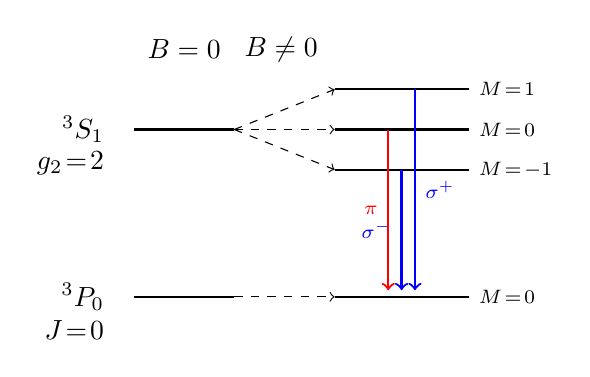
\begin{tikzpicture}[scale=0.85]
    % 上能级 3S1
    \node[left] at (-0.3,4) {${}^3S_1$};
    \node[left] at (-0.3,3.5) {$g_2\!=\!2$};
    \draw[thick] (0,4) -- (1.5,4);
    \draw[thick] (3,4.6) -- (5,4.6) node[right]{\scriptsize$M\!=\!1$};
    \draw[thick] (3,4.0) -- (5,4.0) node[right]{\scriptsize$M\!=\!0$};
    \draw[thick] (3,3.4) -- (5,3.4) node[right]{\scriptsize$M\!=\!-1$};
    \draw[->,dashed] (1.5,4) -- (3,4.6);
    \draw[->,dashed] (1.5,4) -- (3,4.0);
    \draw[->,dashed] (1.5,4) -- (3,3.4);
    % 下能级 3P0
    \node[left] at (-0.3,1.5) {${}^3P_0$};
    \node[left] at (-0.3,1.0) {$J\!=\!0$};
    \draw[thick] (0,1.5) -- (1.5,1.5);
    \draw[thick] (3,1.5) -- (5,1.5) node[right]{\scriptsize$M\!=\!0$};
    \draw[->,dashed] (1.5,1.5) -- (3,1.5);
    % 跃迁
    \draw[->,blue,thick] (4.0,3.4) -- (4.0,1.6) node[midway,left]{\scriptsize$\sigma^-$};
    \draw[->,red,thick] (3.8,4.0) -- (3.8,1.6) node[midway,left]{\scriptsize$\pi$};
    \draw[->,blue,thick] (4.2,4.6) -- (4.2,1.6) node[midway,right]{\scriptsize$\sigma^+$};
    % B标注
    \node at (2.2,5.2) {$B\neq 0$};
    \node at (0.75,5.2) {$B=0$};
  \end{tikzpicture}
  \end{center}

  偏振态：横向观察时$\pi$为平行磁场的线偏振光，$\sigma^\pm$为垂直磁场的线偏振光；纵向观察时$\pi$不可见，$\sigma^+$为右旋圆偏振光，$\sigma^-$为左旋圆偏振光。

  \textbf{(b) \SI{435.8}{nm}（${}^3S_1 \to {}^3P_1$）}

  上能级${}^3S_1$：$J=1,\;g_2=2$，$M=-1,0,1$；
  下能级${}^3P_1$：$L=1,\;S=1,\;J=1$，$g_1=3/2$，$M=-1,0,1$。

  注意：$\Delta J=0$时，$M_2=0 \to M_1=0$的$\pi$跃迁被\textbf{禁戒}。

  各允许跃迁及裂距：
  \begin{itemize}
    \item $\pi$（$\Delta M=0$）：$M=\pm 1$，$\Delta\tilde{\nu}=M(g_2\!-\!g_1)\tilde{L}=\pm\frac{1}{2}\tilde{L}$，共2条；
    \item $\sigma^+$（$\Delta M=+1$）：
      \begin{itemize}
        \item $M_1=-1 \to M_2=0$：$\Delta\tilde{\nu}=\frac{3}{2}\tilde{L}$
        \item $M_1=0 \to M_2=1$：$\Delta\tilde{\nu}=2\tilde{L}$
      \end{itemize}
    \item $\sigma^-$（$\Delta M=-1$）：
      \begin{itemize}
        \item $M_1=1 \to M_2=0$：$\Delta\tilde{\nu}=-\frac{3}{2}\tilde{L}$
        \item $M_1=0 \to M_2=-1$：$\Delta\tilde{\nu}=-2\tilde{L}$
      \end{itemize}
  \end{itemize}
  共6条谱线，位于$-2\tilde{L},\;-\frac{3}{2}\tilde{L},\;-\frac{1}{2}\tilde{L},\;+\frac{1}{2}\tilde{L},\;+\frac{3}{2}\tilde{L},\;+2\tilde{L}$。

  \begin{center}
  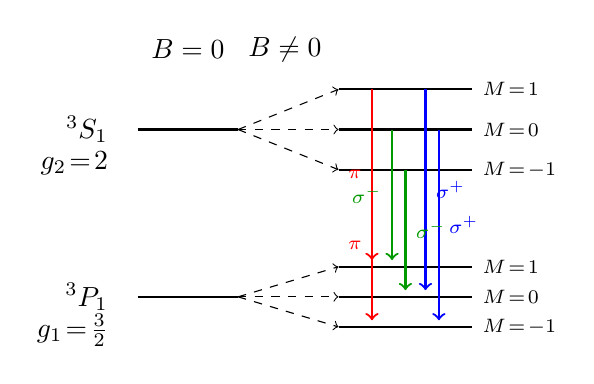
\begin{tikzpicture}[scale=0.85]
    % 上能级 3S1
    \node[left] at (-0.3,4) {${}^3S_1$};
    \node[left] at (-0.3,3.5) {$g_2\!=\!2$};
    \draw[thick] (0,4) -- (1.5,4);
    \draw[thick] (3,4.6) -- (5,4.6) node[right]{\scriptsize$M\!=\!1$};
    \draw[thick] (3,4.0) -- (5,4.0) node[right]{\scriptsize$M\!=\!0$};
    \draw[thick] (3,3.4) -- (5,3.4) node[right]{\scriptsize$M\!=\!-1$};
    \draw[->,dashed] (1.5,4) -- (3,4.6);
    \draw[->,dashed] (1.5,4) -- (3,4.0);
    \draw[->,dashed] (1.5,4) -- (3,3.4);
    % 下能级 3P1
    \node[left] at (-0.3,1.5) {${}^3P_1$};
    \node[left] at (-0.3,1.0) {$g_1\!=\!\frac{3}{2}$};
    \draw[thick] (0,1.5) -- (1.5,1.5);
    \draw[thick] (3,1.95) -- (5,1.95) node[right]{\scriptsize$M\!=\!1$};
    \draw[thick] (3,1.50) -- (5,1.50) node[right]{\scriptsize$M\!=\!0$};
    \draw[thick] (3,1.05) -- (5,1.05) node[right]{\scriptsize$M\!=\!-1$};
    \draw[->,dashed] (1.5,1.5) -- (3,1.95);
    \draw[->,dashed] (1.5,1.5) -- (3,1.50);
    \draw[->,dashed] (1.5,1.5) -- (3,1.05);
    % 跃迁 π (ΔM=0, M=±1 only, M=0→0 forbidden)
    \draw[->,red,thick] (3.5,4.6) -- (3.5,2.05) node[midway,left]{\scriptsize$\pi$};
    \draw[->,red,thick] (3.5,3.4) -- (3.5,1.15) node[midway,left]{\scriptsize$\pi$};
    % 跃迁 σ+ (ΔM=+1)
    \draw[->,blue,thick] (4.5,4.0) -- (4.5,1.15) node[midway,right]{\scriptsize$\sigma^+$};
    \draw[->,blue,thick] (4.3,4.6) -- (4.3,1.60) node[midway,right]{\scriptsize$\sigma^+$};
    % 跃迁 σ- (ΔM=-1)
    \draw[->,green!60!black,thick] (4.0,3.4) -- (4.0,1.60) node[midway,right]{\scriptsize$\sigma^-$};
    \draw[->,green!60!black,thick] (3.8,4.0) -- (3.8,2.05) node[midway,left]{\scriptsize$\sigma^-$};
    % B标注
    \node at (2.2,5.2) {$B\neq 0$};
    \node at (0.75,5.2) {$B=0$};
  \end{tikzpicture}
  \end{center}

  偏振态与(a)相同：横向观察时$\pi$为平行磁场的线偏振光（2条），$\sigma$为垂直磁场的线偏振光（4条）；纵向观察时$\pi$不可见，$\sigma^+$为右旋圆偏振，$\sigma^-$为左旋圆偏振。
\end{enumerate}

%%%%%%%%%%%%%%%%%%%%%%%%%%%%%%%%%%%%%%%%%%%%%%%%%%%%%%%%%%%%
\clearpage
\onecolumn
\section*{参考文献}

\begin{enumerate}[label={[\arabic*]}]
  \item 褚圣麟. 原子物理学[M]. 北京：人民教育出版社，1979.
  \item 毋国光，战元龄. 光学[M]. 北京：人民教育出版社，1978.
  \item 徐克尊，陈宏芳，周子舫. 近代物理学[M]. 北京：高等教育出版社，1993.
  \item 廖红波. 塞曼效应实验[J]. 物理实验，2017，37(7)：25--31.
  \item 杨福家. 原子物理学[M]. 4版. 北京：高等教育出版社，2008.
\end{enumerate}

\clearpage

\section{教师签名页}

\begin{figure}[H]
  \centering
  
\includegraphics[width=0.6\textwidth]{签名页.jpeg}
  \caption{教师签名页}
\end{figure}

\end{document}
